

\tikzset{every picture/.style={line width=0.75pt}} %set default line width to 0.75pt        

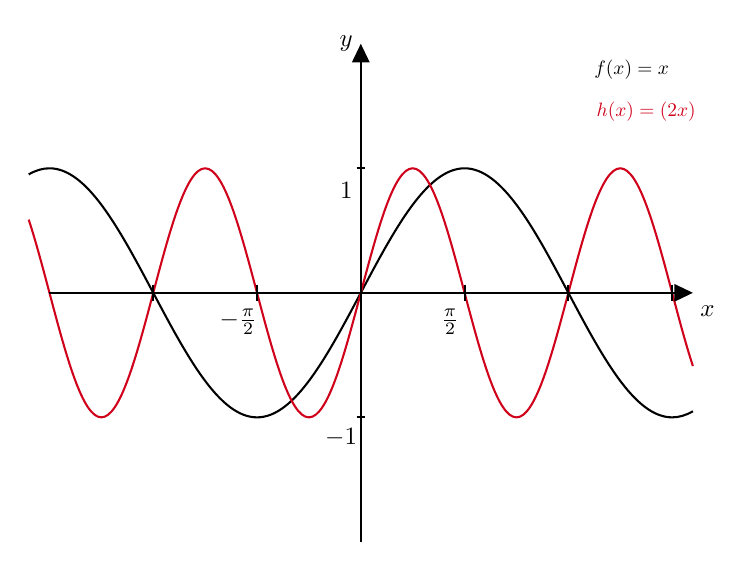
\begin{tikzpicture}[x=0.75pt,y=0.75pt,yscale=-1,xscale=1]
%uncomment if require: \path (0,300); %set diagram left start at 0, and has height of 300

%Shape: Wave [id:dp94416819522044] 
\draw   (180,102.94) .. controls (183.26,101.04) and (186.58,100) .. (190,100) .. controls (208.1,100) and (223.69,129.26) .. (240,160) .. controls (256.31,190.74) and (271.9,220) .. (290,220) .. controls (308.1,220) and (323.69,190.74) .. (340,160) .. controls (356.31,129.26) and (371.9,100) .. (390,100) .. controls (408.1,100) and (423.69,129.26) .. (440,160) .. controls (456.31,190.74) and (471.9,220) .. (490,220) .. controls (493.42,220) and (496.74,218.96) .. (500,217.06) ;
%Shape: Wave [id:dp05495114548578883] 
\draw  [color={rgb, 255:red, 208; green, 2; blue, 27 }  ,draw opacity=1 ] (180,124.73) .. controls (183.35,134.95) and (186.64,147.35) .. (190,160) .. controls (198.15,190.74) and (205.95,220) .. (215,220) .. controls (224.05,220) and (231.85,190.74) .. (240,160) .. controls (248.15,129.26) and (255.95,100) .. (265,100) .. controls (274.05,100) and (281.85,129.26) .. (290,160) .. controls (298.15,190.74) and (305.95,220) .. (315,220) .. controls (324.05,220) and (331.85,190.74) .. (340,160) .. controls (348.15,129.26) and (355.95,100) .. (365,100) .. controls (374.05,100) and (381.85,129.26) .. (390,160) .. controls (398.15,190.74) and (405.95,220) .. (415,220) .. controls (424.05,220) and (431.85,190.74) .. (440,160) .. controls (448.15,129.26) and (455.95,100) .. (465,100) .. controls (474.05,100) and (481.85,129.26) .. (490,160) .. controls (493.36,172.65) and (496.65,185.05) .. (500,195.27) ;
%Straight Lines [id:da13690129851328403] 
\draw    (190,160) -- (498,160) (240,156) -- (240,164)(290,156) -- (290,164)(340,156) -- (340,164)(390,156) -- (390,164)(440,156) -- (440,164)(490,156) -- (490,164) ;
\draw [shift={(500,160)}, rotate = 180] [fill={rgb, 255:red, 0; green, 0; blue, 0 }  ][line width=0.75]  [draw opacity=0] (8.93,-4.29) -- (0,0) -- (8.93,4.29) -- cycle    ;

%Straight Lines [id:da021329477973490496] 
\draw    (340,280) -- (340,42) (338,220) -- (342,220)(338,160) -- (342,160)(338,100) -- (342,100) ;
\draw [shift={(340,40)}, rotate = 450] [fill={rgb, 255:red, 0; green, 0; blue, 0 }  ][line width=0.75]  [draw opacity=0] (8.93,-4.29) -- (0,0) -- (8.93,4.29) -- cycle    ;


% Text Node
\draw (470.5,52.5) node [scale=0.7]  {$f( x) =\sen x$};
% Text Node
\draw (383,174) node [scale=0.9,color={rgb, 255:red, 0; green, 0; blue, 0 }  ,opacity=1 ]  {$\frac{\pi }{2}$};
% Text Node
\draw (281,174) node [scale=0.9,color={rgb, 255:red, 0; green, 0; blue, 0 }  ,opacity=1 ]  {$-\frac{\pi }{2}$};
% Text Node
\draw (333,110.5) node [scale=0.9]  {$1$};
% Text Node
\draw (330.5,229.5) node [scale=0.9]  {$-1$};
% Text Node
\draw (477.5,72.5) node [scale=0.7,color={rgb, 255:red, 208; green, 2; blue, 27 }  ,opacity=1 ]  {$h( x) =\sen ( 2x)$};
% Text Node
\draw (507,169) node [scale=0.9]  {$x$};
% Text Node
\draw (333,40) node [scale=0.9]  {$y$};


\end{tikzpicture}
